%%% Choose between 16:9 and 4:3 format by commenting out/uncommenting one of the following lines:
\documentclass[aspectratio=169]{beamer} % 16:9
% \documentclass{beamer} % 4:3

%=========================================================================================================================

\usepackage[english]{babel}     % English language
\usepackage[latin1]{inputenc}   % Input encoding
\usepackage{tikz}               % For creating graphics
\usepackage{url}                % For including urls
\usepackage{tabularx}           % For better tables

\usetheme{aig}                  % Set beamer theme

%=========================================================================================================================
\title{Qualit\"at von Wikipedia-Artikeln}

\author[R. Suxdorf et al.]{Robin Suxdorf, Johannes Kr\"amer, Alexander Kunze, Sebastian Bunge, Emmanuelle Steenhof}
\institute{Artificial Intelligence Group,\\
University of Hagen, Germany}
\date{17. Dezember 2024}
%=========================================================================================================================
\logo{
\includegraphics[width=3cm]{figures/logoaig.png}}
%=========================================================================================================================

\begin{document}

%=========================================================================================================================

\begin{frame}
  \titlepage
\end{frame}
\nologo



% \begin{frame}{Blocks}
%    \begin{block}{Block}
%        This is a regular block.
%        \begin{itemize}
%            \item This is an item in a block.
%        \end{itemize}
%    \end{block}

%    \begin{alertblock}{Block}
%        This is an alert block.
%        \begin{itemize}
%            \item This is an item in an alert block.
%        \end{itemize}
%    \end{alertblock}

%    \begin{exampleblock}{Block}
%        This is an example block.
%        \begin{itemize}
%            \item This is an item in an example %block.
%        \end{itemize}
%    \end{exampleblock}
% \end{frame}


% \subsection{Subsection}

% \begin{frame}{Highlighting Text}
%   We can \highlight{highlight} text. There are also %a \darkhighlight{darker} option, and a %\yellowhighlight{yellow} option.\\
%    The same options are also available in math mode: $\mathhighlight{a} + \darkmathhighlight{b} = \yellowmathhighlight{c}$
% \end{frame}


% \appendix

% \section{Appendix}

% \begin{frame}{Appendix}
%    This is an appendix.
%    \begin{itemize}
%        \item Page numbers start from the beginning.
%    \end{itemize}
% \end{frame}

\section{Organisation}
\begin{frame}
  Organisation
  \begin{itemize}
    \item Kommunikation: Discord Channel
    \item Gespr\"achstermine: Alle zwei Wochen
    \item Aufgabenaufteilung: Ein Leiter pro Thema
  \end{itemize}
\end{frame}

\section{Problemstellung}
\begin{frame}
  Problemstellung
  \begin{itemize}
    \item Modell finden, welches in der Lage ist Wikipediaartikel aufgrund ihrer Qualit\"at auszusortieren und zu klassifizieren, weshalb sie schlecht sind.
  \end{itemize}
\end{frame}

\section{Datenvorbereitung und Analyse}
\begin{frame}
  Datenvorbereitung und Analyse
  \begin{itemize}
    \item Beschreibung der Daten:
          \begin{itemize}
           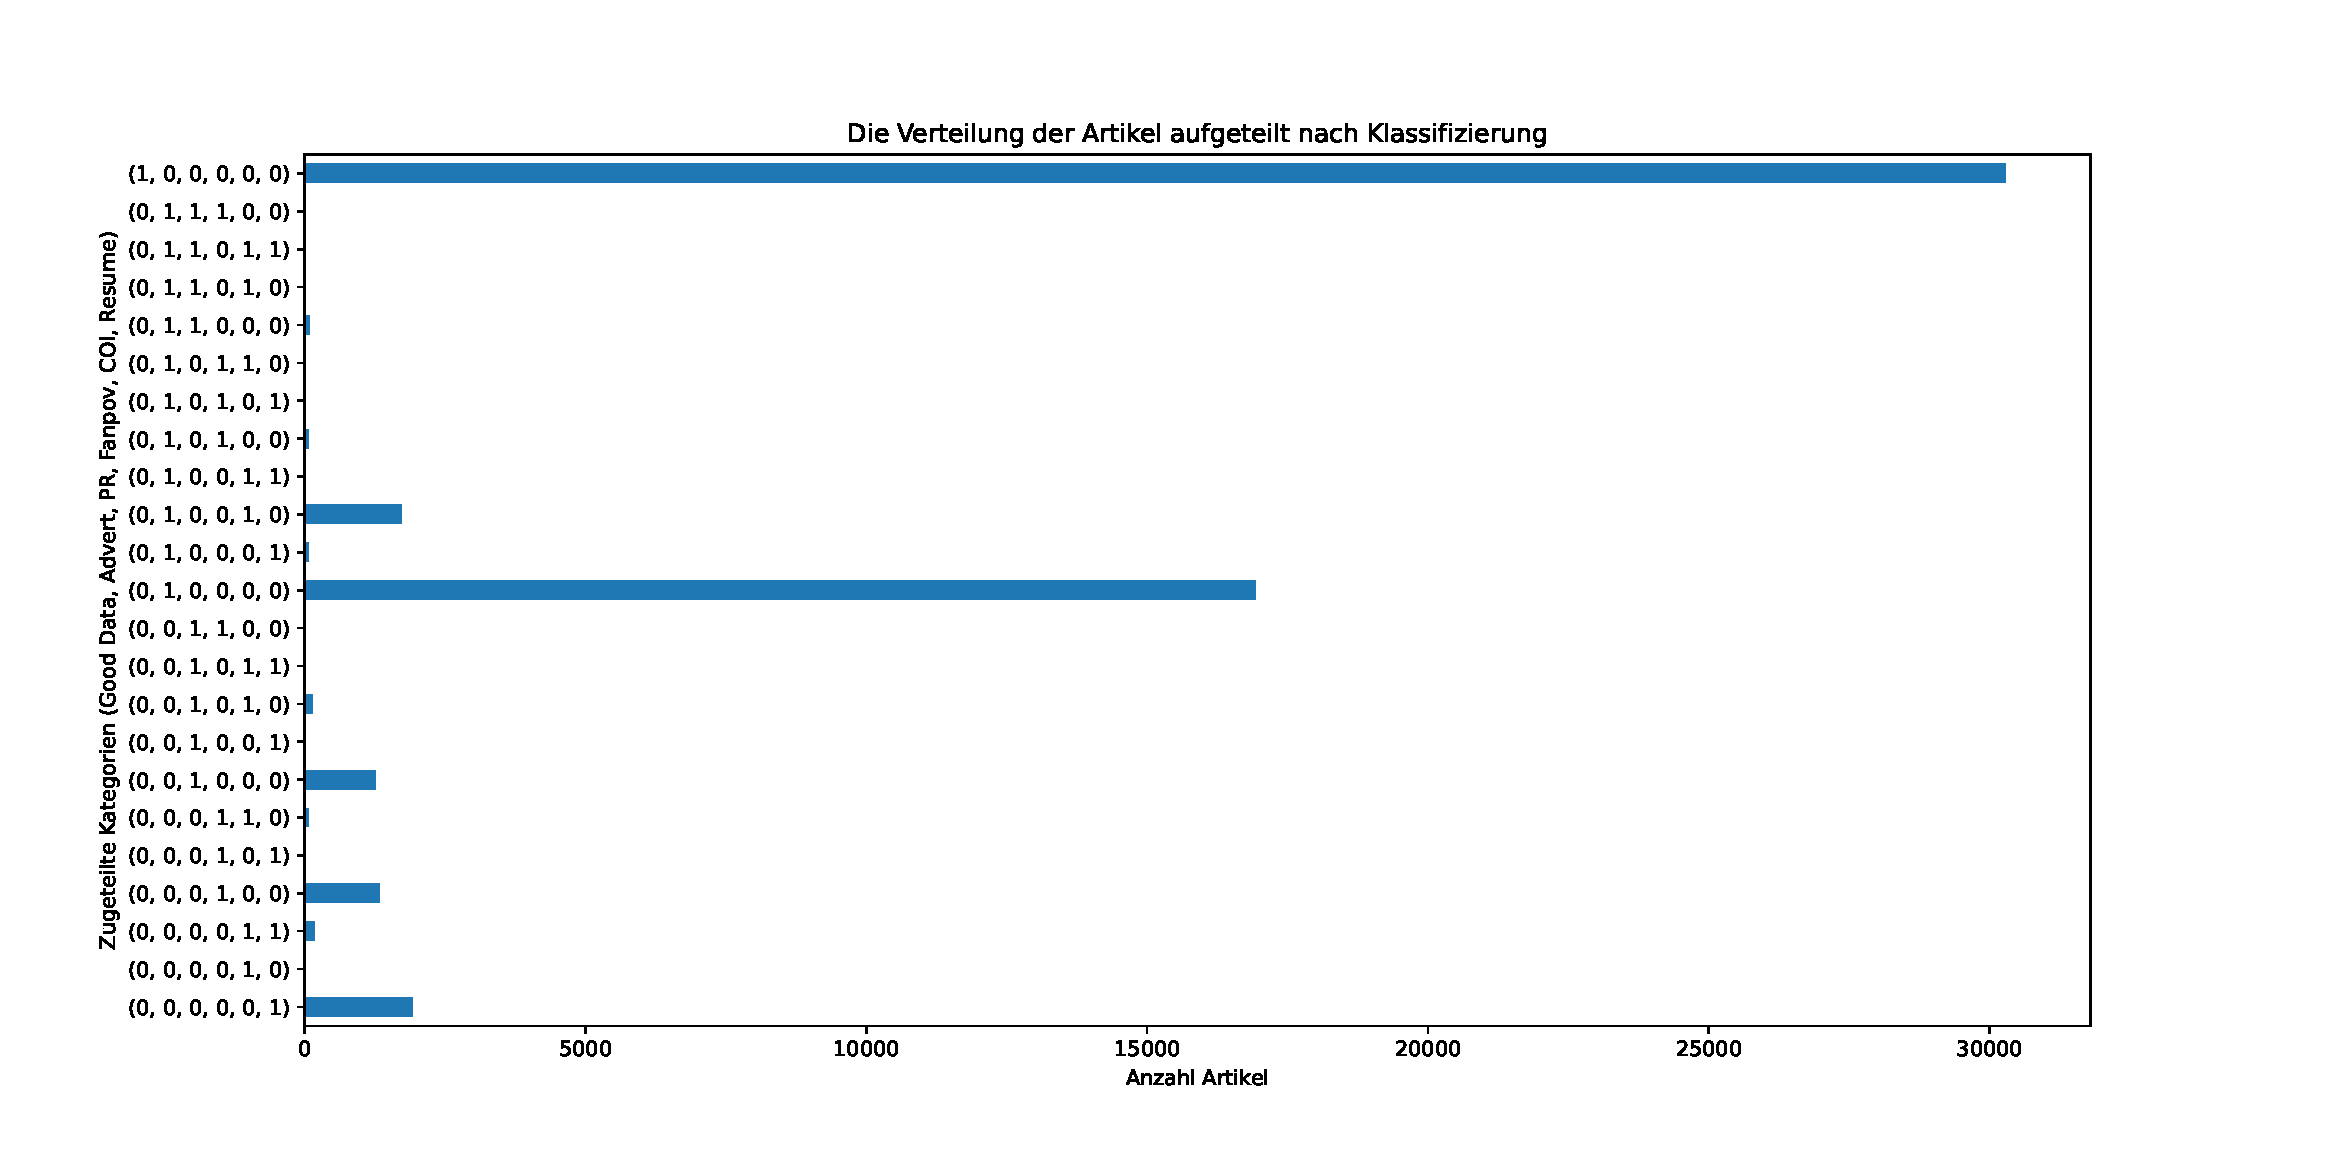
\includegraphics[width=10cm]{figures/GrafikVerteilungKlassenH.eps}
          \end{itemize}
    \item Datens\"atze die Hinzugezogen werden:
          \begin{itemize}
            \item  Offizielle Artikel, die von Wikipedia monatlich rausgeworfen werden
            \item Versuche mit Data Augmentation werden gemacht
            \item Suche nach weiteren Websites: Fanpages, Wissenschaftliche Artikel usw.
          \end{itemize}
  \end{itemize}
\end{frame}


\section{Fortschritt Implementierung Modelle}
\begin{frame}
  SVM
  \begin{itemize}
    \item Leiter:...
    \item Bisherige Arbeit: ...
    \item Resultate: ..
    \item Aufgetauchte Probleme: ...
    \item N\"achste Schritte: ...
  \end{itemize}
\end{frame}

\subsection{Logistische Regression}
\begin{frame}
  Logistische Regression
  \begin{itemize}
    \item Leiter:...
    \item Bisherige Arbeit: ...
    \item Resultate: ..
    \item Aufgetauchte Probleme: ...
    \item N\"achste Schritte: ...
  \end{itemize}
\end{frame}

\subsection{Bayes Klassifikator}
\begin{frame}
  Bayes Klassifikator
  \begin{itemize}
    \item Leiter:...
    \item Bisherige Arbeit: ...
    \item Resultate: ..
    \item Aufgetauchte Probleme: ...
    \item N\"achste Schritte: ...
  \end{itemize}
\end{frame}

\subsection{CNN}
\begin{frame}
  CNN
  \begin{itemize}
    \item Leiter:...
    \item Bisherige Arbeit: ...
    \item Resultate: ..
    \item Aufgetauchte Probleme: ...
    \item N\"achste Schritte: ...
  \end{itemize}
\end{frame}

\subsection{5.Ansatz}
\begin{frame}
  Ideen 5. Ansatz
  \begin{itemize}
    \item Graphen der Beziehungen der Daten
    \item Imitierung der Embeddings durch Gram-Schmidt-Verfahren - Erste Versuche bereits gelaufen
    \item Vortrainierte Embeddings verwenden, als Eingabe f\"ur andere Methoden des maschiniellen Lernens.
  \end{itemize}
\end{frame}

\section{Zusammenfassung}
\begin{frame}
  Zusammenfassung
  \begin{itemize}
    \item Gemachte Arbeit
    \item Probleme
    \item N\"achste Schritte
    \begin{itemize}
    \item Weitere Datens\"atze finden/erg\"anzen
    \item Weitere Ideen f\"ur f\"unften Ansatz ausdenken bzw. weiter testen.
    \end{itemize}
  \end{itemize}
\end{frame}

\end{document}
